\documentclass[12pt,letterpaper]{article}
\usepackage{fullpage}
\usepackage[top=2cm, bottom=4.5cm, left=2.5cm, right=2.5cm]{geometry}
\usepackage{amsmath,amsthm,amsfonts,amssymb,amscd}
\usepackage{lastpage}
\usepackage{enumerate}
\usepackage{fancyhdr}
\usepackage{mathrsfs}
\usepackage{xcolor}
\usepackage{graphicx}
\usepackage{listings}
\usepackage{hyperref}
\usepackage{float}

\hypersetup{%
  colorlinks=true,
  linkcolor=blue,
  linkbordercolor={0 0 1}
}
 
\renewcommand\lstlistingname{Algorithm}
\renewcommand\lstlistlistingname{Algorithms}
\def\lstlistingautorefname{Alg.}

\lstdefinestyle{Python}{
    language        = Python,
    frame           = lines, 
    basicstyle      = \footnotesize,
    keywordstyle    = \color{blue},
    stringstyle     = \color{green},
    commentstyle    = \color{red}\ttfamily
}

\setlength{\parindent}{0.0in}
\setlength{\parskip}{0.05in}

% Edit these as appropriate
\newcommand\course{He-6 CRES Project}
\newcommand\hwnumber{CRES Kassiopeia Results}                  % <-- homework number
\newcommand\NetIDa{Alexander Allen}           % <-- NetID of person #1

\pagestyle{fancyplain}
\headheight 35pt
\lhead{\NetIDa}
\chead{\textbf{\Large \hwnumber}}
\rhead{\course \\ \today}
\lfoot{}
\cfoot{}
\rfoot{\small\thepage}
\headsep 1.5em

\begin{document}


\section{Introduction}

We present results for simulations using the Kassiopeia software developed for the Katrin experiment. Source code for the Kassiopeia project can be found \href{https://github.com/KATRIN-Experiment/Kassiopeia}{here}. 

These simulations establish a cylindrical experimentation space with the z-axis defined along the length of the cylinder. The cylinder is $60~$cm in length and has a radius of $0.058~$cm representing a wave guide.

At the center of the geometry there is a particle generator which generates electrons with kinetic energy of $100~$keV and an isotropic velocity distribution into a $2\pi$ solid angle in the positive z direction.

\subsection*{Contents}

This paper contains a number of experiments first validating the Kassiopeia particle track integrator, then validating our simulation design, and finally validating our proposed cutout design

\begin{itemize}
    \item \textbf{Constant B-Field Simulation} (Validate Integrator Precision)
    \item \textbf{Constant E/B-Field Simulation} (Validate Particle Drift)
    \item \textbf{Trapping Field Simulation} (Validate Magnetic Bottle Design)
    \item \textbf{Constant E-Field Sweep} (Validate Approximate Emptying Time)
    \item \textbf{Simulated E-Field Sweep} (Validate Complete Proposed Geometry)
\end{itemize}

\subsection*{Summary}

We first analyze the cyclotron motion of these generated particles under the application of a $1~$T magnetic field along the z-axis. Here we verify that conservation of energy is maintained, verify that the larmor radius is what we expect, and determine that the precision of the simulation is well within our tolerances by predicting the final location using the initial conditions and comparing it to the simulation results. 

Next, we analyze the same cyclotron motion with the addition of an E-field that creates electron drift. We calculate the location we expect to find the center of rotation of the electrons and then compare that to the center that is determined from the simulation. We then compute the theoretical drift velocity, adjust our predictions and calculate a second set of errors. We plot both of these errors over time and find that the predictions without accounting for drift have unbounded error while the predictions using the theoretical drift velocity have low and well bounded error values over time allowing us to confirm our simulation is behaving as expected. 

Next, we add a solenoidal magnetic field to the simulation to create an electron trap. We calculate the critical pitch angle for the electron to be trapped and we calculate the resulting trapping fraction of the population of electrons. We verify that larger pitch angles result in lower oscillation times and smaller magnetron motion. 

Next, we add an electric field to the trapping geometry to model electron drift in the trap. We extract the time it takes trapped electrons to reach the edge of the geometry and plot that in a histogram. We determine that the emptying time for electrons in the trap generally resides between 5 and 50 nanoseconds and conclude that the electric field applied in the simulation is adequate for emptying the trap of charged particles in a reasonable time frame without the need to remove the magentic field. 

Finally, we simulate this geometry in ANSYS Maxwell 3D with our proposed cutout in place and validate that the cutout does not interfere with waveguide operation in the frequencies of interest by coupling to degenerate modes. We then apply $1000~$V over the cutout and simulate the electric field which we then visualize and then export to Kassiopeia where we run the emptying time simulation again. Here we find that the particles generally leave within $10~$ns thus validating our cutout design as an operable solution to empty the trap.

\section{Constant B-Field}

In the first experiment a constant magnetic field of magnitude 1 Tesla is applied globally along the positive z-axis. The active geometry is a cylinder of radius $0.0058~$m and length $0.6~$m oriented along the z-axis and centered at the origin.

\subsection{Conservation of Energy}

Firstly we ensure that conservation of energy is held by plotting a histogram of change in kinetic energy from beginning to the end of the simulation for the population of electrons simulated. In an ideal scenario this is zero, thus this is a indicator of the error we are seeing in the built-in integrator. 

    \begin{figure}[H]
    \centering
    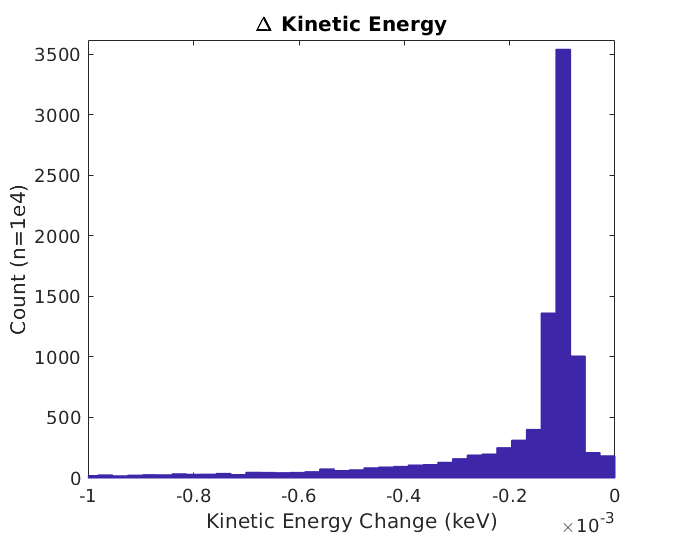
\includegraphics[width=0.7\linewidth]{img/ke.png}
    \caption{Change in kinetic energy}
    \end{figure}
    
We see here that the error generally lies less than $2\times10^{-4}~$eV which is a reasonable range given the $100\times10^{3}~$eV initial kinetic energy the electrons start with.

\subsection{Arrival Time Distribution}

Next we analyze the arrival times of the electrons to the end of the geometry. This is the time it takes for the electron to travel from its incident location to the end of the geometry 30cm from the generator. We use this metric to verify that the generator is isotropically distributing the initial momentum vector of the electrons as this assumption drives many other conclusions we can draw from this simulation. 

We use the arrival time to calculate a $v_z$ value by

\[ v_z = \frac{0.3}{t} \]

Given the kinetic energy of $100~$keV we can calculate the total velocity of the elctron using the relativistic form of kinetic energy

\[ \frac{v}{c} = \sqrt{1 - \frac{1}{(K/m_0 + 1)^2}} \] = 0.5482


thus we can compute the ratio of the z-component velocity to the total velocity by

\[ \frac{v_z}{v} = \frac{v_z}{0.5482c} \]

The isotopic distribution is defined as a uniform distribution over $cos(\theta)$ from zero to one.

\[ cos(\theta) = \frac{v_z}{v} = \frac{v_z}{0.5482c} \]

Thus, we expect that the distribution of $\frac{v_z}{v}$ across the population of electrons be uniform.

    \begin{figure}[H]
    \centering
    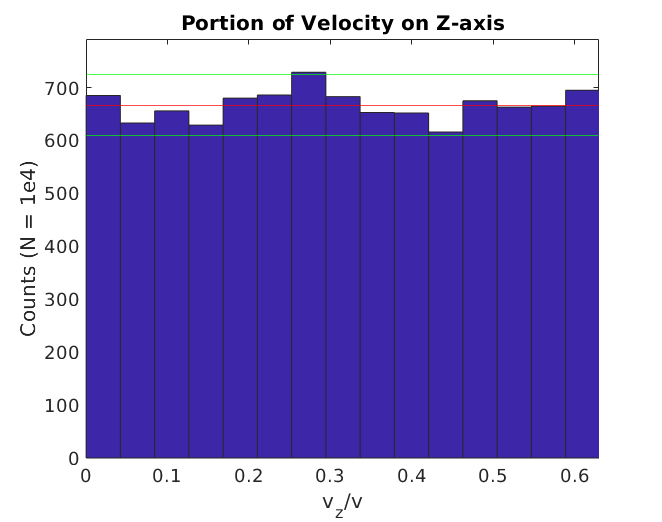
\includegraphics[width=0.7\linewidth]{img/arrival.png}
    \caption{Distribution of velocities parallel to the geometry}
    \end{figure}
    
We can see that this population sample shown here is generally uniform and thus the distribution of particle trajectories is likely isotropic. 

One feature of this histogram is that the deviation from the mean / uniform value increases as the velocity of the particle increases in the z direction. Due to the nature of the inverse function and floating point math in the simulation system, very small arrival times (which correspond to the higher velocities) are much more sensitive to small floating point errors and small errors originating from the numerical integrator (8th order Runge-Kutta) which is why we see the greater deviation. 

However, it can also be observed that these deviations are largely a factor of the binning of the histogram and that binning at larger intervals smooths out these deviations which supports the conclusion that the observed deviance is mostly random error rather than systematic. Additionally, the red and green lines on the chart represent the mean and 95\% point of the count value and all counts fall within these bounds suggesting that our deviation from uniform is Gaussian in nature.

\subsection{Larmor Radius}

Next, we analyze the Larmor radius of the particles as they travel down the geometry. We can predict the Larmor radius using the initial conditions of the particle by

\[ v_{\perp} = v_z\frac{p_x^2 + p_y^2}{p_x^2 + p_y^2 + p_z^2} \]
\[ \gamma = \frac{1}{\sqrt{1 - 0.5482^2}} = 1.1957 \]
\[ r = \frac{\gamma mv_\perp}{qB}  \]

To locate the center of rotation we perform a 90 degree rotation of the initial tangential momentum vector of the electron to create a vector pointed towards the center of rotation from the origin (incident location). We then set the magnitude of that vector to the Larmor radius to create a vector which points from the incident location to the rotational center.

For each step in the simulated particles trajectory we perform this same computation and calculate the center of rotation. Then, for each step we calculate the displacement of the calculated center from the initial center location. 

We collect this displacement error value for all recorded steps of all particles and present a histogram of these error values. We also present a plot of the displacement over time for a sample particle to show variation over time.

    \begin{figure}[H]
    \centering
    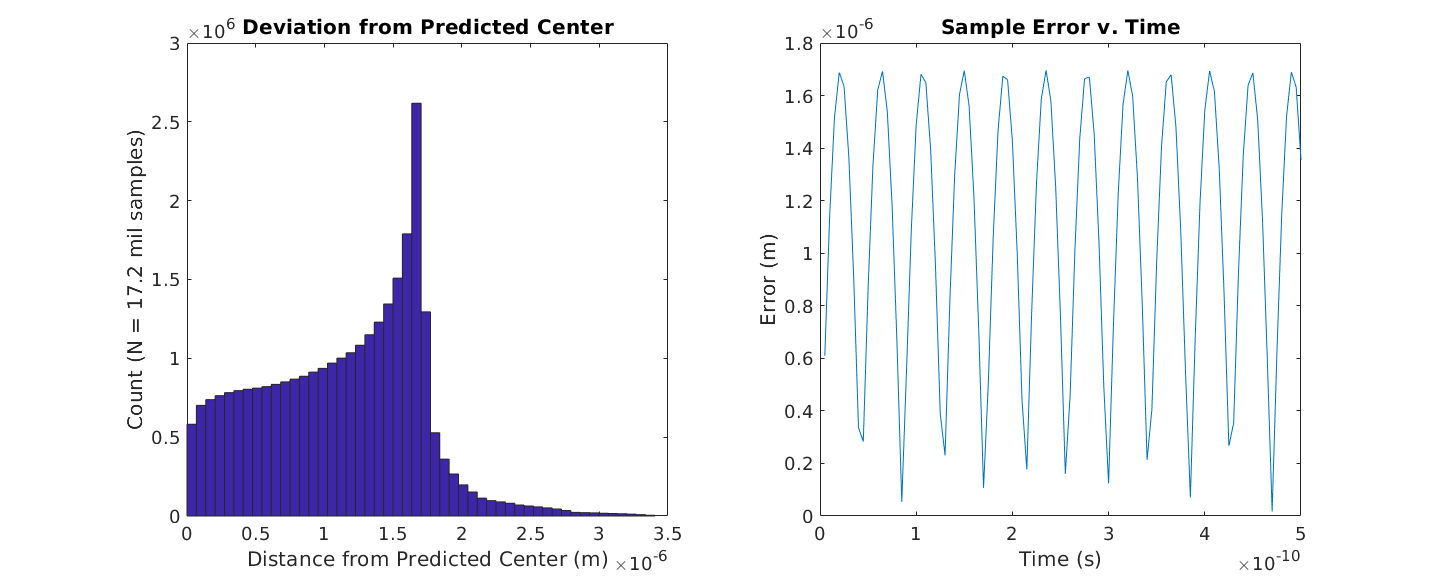
\includegraphics[width=\linewidth]{img/larmor.png}
    \caption{Larmor Radius Error}
    \end{figure}
    

Error values peak at $1.5~\mu m$ and drop off significantly at $2~\mu m$ which is an acceptably low value. This shows that the motion of the particle is indeed circular, tangent to its initial position, and matches the trajectory and velocity we expect given the simulation conditions. 

We also see that the transient error for the sample particle is sinusoidal in nature and is oscillating near the desired value rather than growing in a direction. This suggests that the predicted larmor radius slightly varies from the simulated value but the center of not rotation is not significantly drifting during particle travel. 

We also visualize the x-y projection of the trajectories of the particles as an additional layer of validation. The simulation boundary is super-imposed on this plot for visualization purposes. 

    \begin{figure}[H]
    \centering
    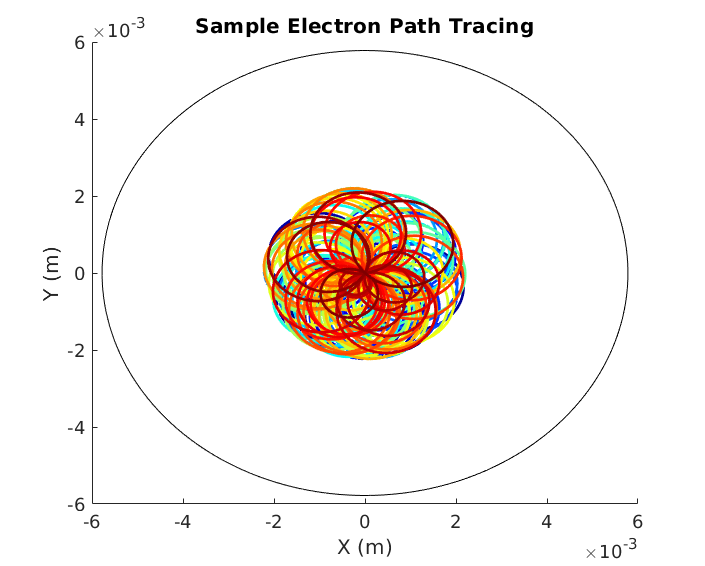
\includegraphics[width=0.9\linewidth]{img/track.png}
    \caption{Particle track visualization}
    \end{figure}

\subsection{Phase}
    
Finally, to evaluate the precision with which the simulation calculates particle paths, we use the initial conditions of the particle to predict the trajectory and final coordinates of the electron. To do this we once again evaluate the center of rotation using the computed Larmor radius and we also use the initial momentum to calculate the angular frequency around that center. We then use the momentum in the z direction to predict the arrival time of the particle and use that in conjunction with the angular frequency to predict the relative position of the particle around its center when it terminates at the end of the geometry. 

We then look at the final position of the particle given by the simulation and compare it to the prediction. The value we compute for these positions is the cumulative displacement in radians around the center of the cyclotron motion from the initial condition to the final condition. 

We construct a histogram of errors consisting of the difference between the predicted phase and the phase reported by the simulation.

    \begin{figure}[H]
    \centering
    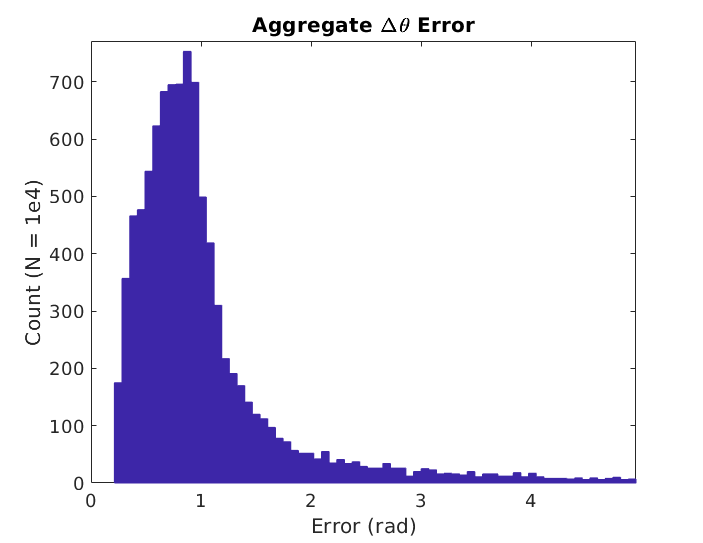
\includegraphics[width=0.7\linewidth]{img/phase.png}
    \caption{Phase error}
    \end{figure}
    
These errors are reported in radians and while there are a few outliers the error generally stays below $2~$rad and as such is acceptable to the precision necessary.

\section{ExB Field}

We then modify the simulation in Kassiopeia to include an electric field of magnitude $2\times10^5$~V/m in the negative y direction in the geometry. This will induce a drift velocity for the electrons.

    \begin{figure}[H]
    \centering
    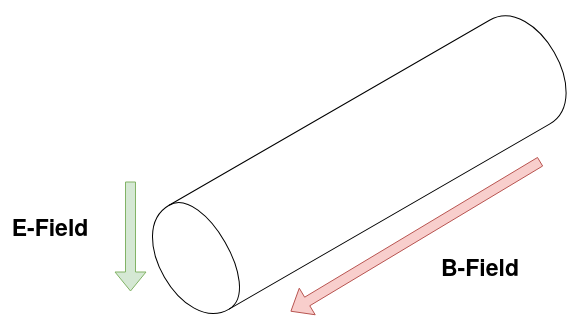
\includegraphics[width=0.8\linewidth]{img/CRES.png}
    \caption{Diagram of Simulation Geometry}
    \end{figure}

To validate this drift is occurring to the magnitude we expect, we repeat the experiment in the previous section that tracks the center of the cyclotron motion of the particles. 

We expect to see displacement values between the initial center point and the final center point corresponding with the drift velocity created by the E-field. To verify this we model the theoretical displacement of the center over time using the following velocity:

\[ v = \frac{E}{B} = \frac{2\times10^5~V/m}{1~T} \]

We then construct a plot of the calculated displacement of all steps over all particles and simultaneously plot the residuals between this plot and the theoretical model

    \begin{figure}[H]
    \centering
    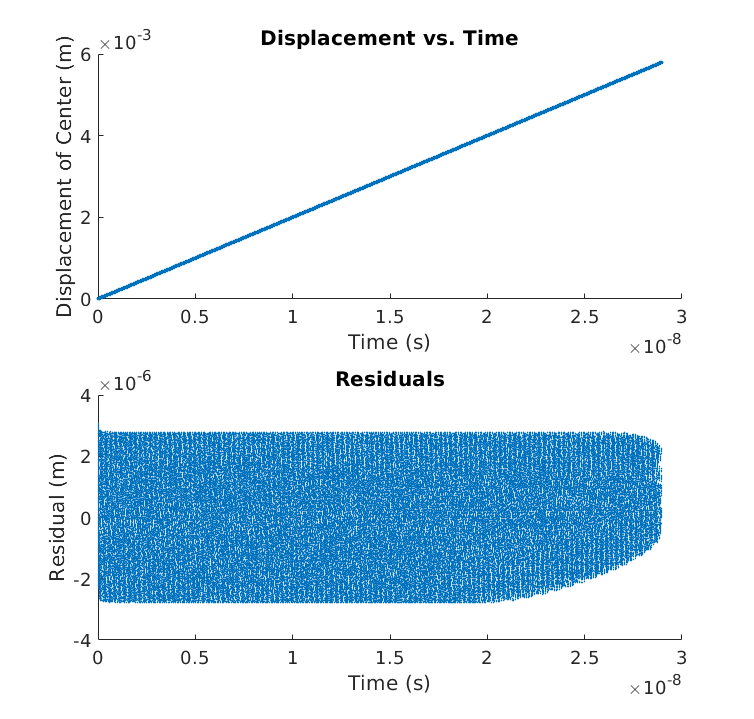
\includegraphics[width=0.9\linewidth]{img/drift.png}
    \caption{Drift Correction}
    \end{figure}

We observe that the error between the simulation and our model is evenly distributed between $-2\times10^{-6}~$m and $2\times10^{-6}~$m which suggests that the error is small (3 orders of magnitude lower than the displacement) and random. From this we conclude that the electrons are drifting at the expected rate and the simulation is performing as intended.

\section{Trapping Field}

Next, we advance the simulation by establishing a solenoidal B-field in the opposite direction of the global $1~$T B-Field around the geometry. The solenoidal field is placed such that it reduces the net magnetic field at the center of the trap to $0.9~$T. 

    \begin{figure}[H]
    \centering
    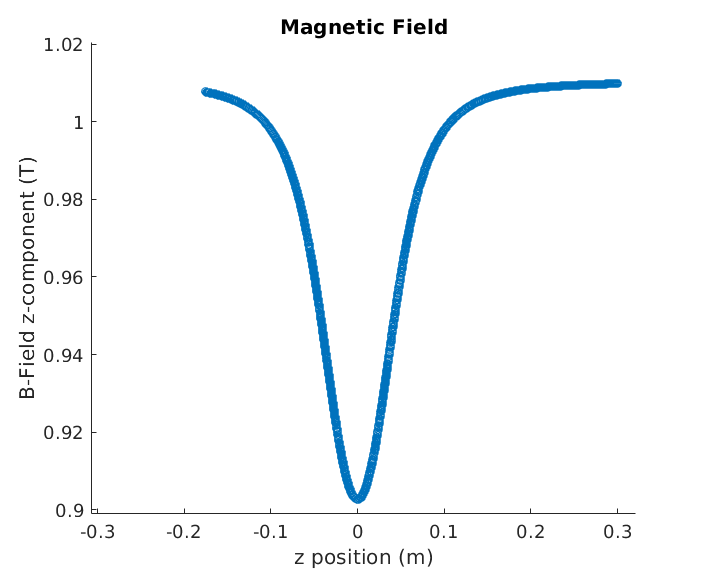
\includegraphics[width=0.7\linewidth]{img/solenoid.png}
    \caption{Visualization of B-Field Experienced by Particles in Trap}
    \end{figure}

This creates a trapping field that should contain electrons with a high ratio of tangential (to the magnetic field) momentum to parallel momentum.

\subsection{Oscillation Behavior}

We expect to see a critical pitch angle (angle of the initial momentum to the positive z-axis) high enough for electrons to be trapped. Using the particle generator at the center of the geometry with an isotropic distribution we can visualize that critical angle and also examine the characteristics of the magnetron motion of the electron. 

    \begin{figure}[H]
    \centering
    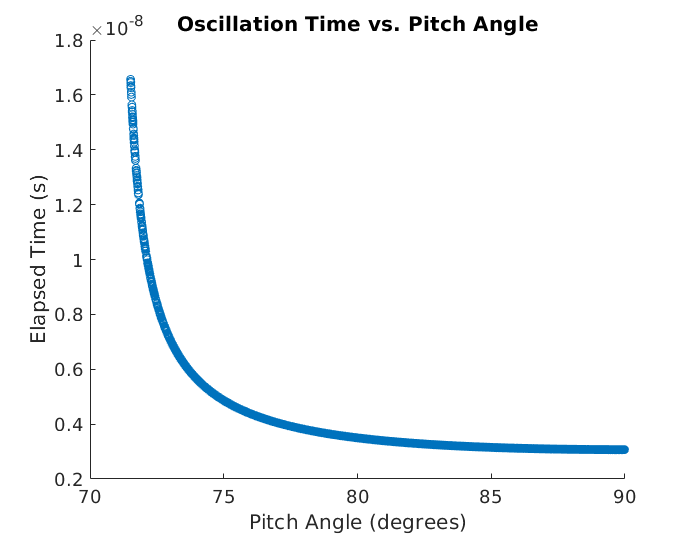
\includegraphics[width=0.7\linewidth]{img/oscillationtime.png}
    \caption{Time of flight of trapped electrons between the classical turning points}
    \end{figure}
    
    \begin{figure}[H]
    \centering
    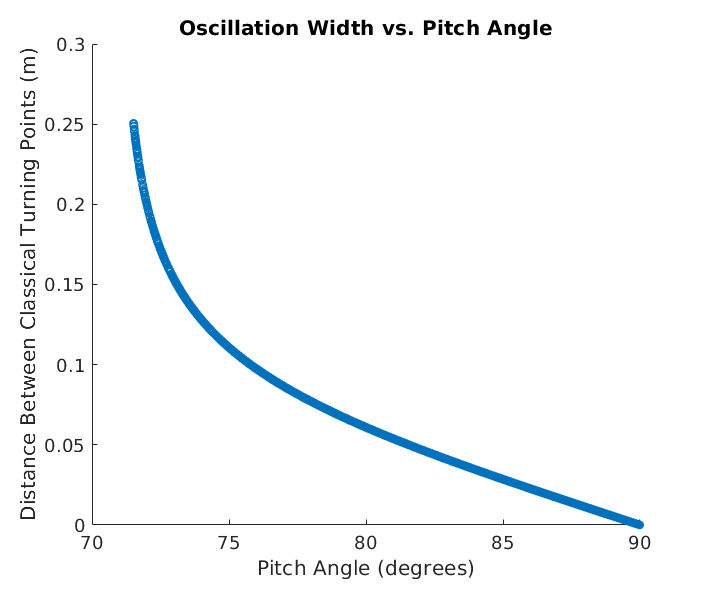
\includegraphics[width=0.7\linewidth]{img/oscillationwidth.png}
    \caption{Width of magnetron motion}
    \end{figure}

The two figures above characterize the magnetron motion of the electrons as it relates to the pitch angle of the electron. We observe that the critical angle is around $71~$degrees where any trapped electron has a greater pitch angle than that. 

We also observe that the oscillation time rapidly decreases with pitch angle to an asymtope of around $35~$ns. The constant time from angles greater than $80~$degrees suggests that the magnetic field is parabolic in this range.

We observe that the oscillation width of the magnetron motion decreases to zero as the pitch angle approaches $90~$degrees as expected. Between these two profiles of the electron motion and the profile of the magnetic field, we conclude that the simulation is behaving as intended. 

\subsection{Trapping Fraction}

To characterize this trap we calculate the trapping fraction, the ratio between the trapped particles and the total number of particles generated. We define a trapped particle as a particle that has existed for more than 10000 simulation steps without encountering a trap boundary (radius of $0.0058~$cm and z position of $\pm30~$cm).

Fist we calculate the theoretical trapping fraction which we will compare to the value measured by the simulation.

To do this, first we calculate the mirror ratio, the ratio between the maximum magnetic field flux density that the electron experiences and the minimum flux density it experiences.

\[ r_m =  \frac{B_{max}}{B_{min}} = \frac{1~T}{0.9~T} = \]

We then calculate the loss cone or the critical ratio between tangential and parallel velocity that will trap the electron

\[ \frac{v_z}{v} = \frac{1}{\sqrt{r_m}} = 0.9454 \]

We can then use this to calculate the critical pitch angle mentioned in the previous section

\[ \theta_c = 90 - cos^{-1}(\frac{v_z}{v}) = 70.9^\circ \]

We can also use this angle to calculate the trapping fraction since we know it is isotropically distributed

\[ k = cos(\theta_c) = 0.326 = 32.6\% \]

By calculating the ratio of particles that survived longer than 10000 steps to the total number of particle generated we calculate the experimental trapping fraction to be $32.1$\% (N = 10000). This is close enough to our theoretical value that we can conclude that the simulation is acting as expected.

We then modify the simulation to generate particles uniformly within the trapping geometry rather than just at the center. We also modify the experiment to generate electrons with energies of $50~$keV to $500~$keV uniformly. This represents a more accurate approach to what would be seen in the CRES experiment. 

We can also calculate a theoretical trapping fraction for this scenario. To do this we construct two separate fractions. One being the fraction arising from the changing energy and the other being the fraction arising from the changing initial z-position.

First we calculate the fraction arising from the changing energies. The larger the energy, the larger the larmor radius will be at the turning points of the electron. This larmor radius cannot cause the electron to collide with the circular waveguide. 

First we derive the expression to calculate the maximum larmor radius from the given energy

\[ v = \sqrt{1 - \frac{1}{(K/m_0 + 1)^2}} \]
\[ \gamma = \frac{1}{\sqrt(1 - v^2)} \]
\[ r_l = \frac{(K + m_0)\sqrt{1 - \frac{1}{(K + m_0)^2}}}{qB} \]

Then we derive the trapping fraction given a larmor radius. We know that any electron generated far enough from the center of the trap that its radius will intersect the geometry will not be trapped.

\[ r_{max} = r - r_l \]

and since we know that the radius from the center the electron is generated at is uniformly generated we can assign a probability of being trapped. 

\[ p = \frac{r - r_l}{r} \]

we can then integrate on this probability across the possible energies. Since the energies are distributed uniformly we can simply calculate the average probability using this integral

\[ k_1 = \frac{1}{K_{HI} - K_{LOW}}\int_{K_{LOW}}^{K_{HI}} \frac{r - \frac{(K + m_0)\sqrt{1 - \frac{1}{(K + m_0)^2}}}{qB}}{r} dK \]

Where $m_0$ is the mass of electrons in kilograms, $q$ is the fundamental charge, and $B$ is the average flux density across the trapping geometry ($0.98~$T). 

Numerically computing this integral yields a trapping fraction of $0.6547$

Next, we calculate the trapping fraction that arises from the particle being generated at different z locations within the trap. This primarily impacts the maximum and minimum magnetic flux density that a given electron experiences and thus alters its apparent mirror ratio and trapping fraction. 

First, we approximate the magnetic flux density in the trap as a parabola from $z=-0.1~$m to $z=0.1~$m with the equation

\[ B = 10z^2 + 0.9 \]

and approximate it as $1~$T elsewhere in the geometry.

Next, we construct the trapping fraction from a given $B$ value as we did earlier in this section. We know this formula is

\[k = cos\left( 90 - cos^{-1}\left( \frac{1}{\sqrt{B_{max}/B_{min}}} \right) \right)\]

We also know the electron has equal probability of being generated in the direction of the center of the trap or the direction of the end of the trap. To account for cases in which the electron travels through the center of the trap and experiences a $B_{min}$ of $0.9~$T we average this with the trapping fraction we computed earlier of $k = 0.326$

\[k = \frac{1}{2} \left[ cos\left( 90 - cos^{-1}\left( \frac{1}{\sqrt{B_{max}/B_{min}}} \right) \right) + 0.326  \right] \]
 
Now we can substitute in the value of $B_{min}$ with the approximation we calculated earlier and integrate from $-0.1~$m to $0.1~$m and divide by $0.6~$m to get the average trapping fraction across the entire geometry. 

\[ k_2 = \frac{1}{0.6}\int_{-0.1}^{0.1}\frac{1}{2} \left[ cos\left( 90 - cos^{-1}\left( \frac{1}{\sqrt{B_{max}/(10z^2 + 0.9)}} \right) \right) + 0.326  \right] dz  \]

Numerically computing this integral yields a trapping fraction of $0.0941$

Finally, we approximate the final trapping fraction by multiplying these individual components together to get a final theoretical trapping fraction of $6.1$\%

Using the same method as earlier we calculate the trapping fraction from the new simulation to be $5.5$\% (N = 10000) which is close enough to our theoretical value to conclude that our assumptions were within reason. 

\section{Trap with Constant E-Field Sweep}
Next, we alter the trap geometry defined in the previous section to include the same E-field defined in section 3. This is an E-field in the negative y direction with a magnitude of $2\times10^5~$V/m. 

Using this geometry, we analyze the time it takes trapped electrons to evacuate the trap. We do this by generating particles using the uniform distribution described in the previous section and examining their behavior.

First, we filter particles that were not trapped by eliminating particles that had a lifetime of less than 100 steps, this eliminates particles whose larmor radius was too large to be contained in the trap initially. We also filter more particles that either had a too great z momentum to be trapped or that were generated too close to the boundary of the trap to be trapped by the B-field.

Taking the particles that remained from the filter method described above, and plotting the time between the generation of these particles and when they encountered the boundary of the geometry yields a histogram of trap emptying times for the population of trapped electrons. 

    \begin{figure}[H]
    \centering
    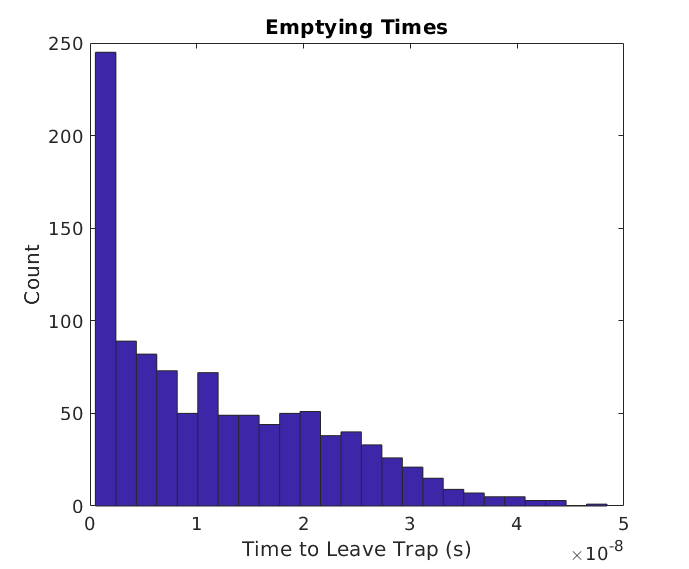
\includegraphics[width=0.7\linewidth]{img/emptying.png}
    \caption{Histogram of Emptying Times (N = 10000)}
    \end{figure}

Here we see that the escape times of the electrons are confined under $50~$ns with a strong peak at zero. This is a good first estimate of the emptying time of the real experiment, and due to the orders of magnitude present we conclude that the proposed electric field will be more than necessary to empty the trap in a reasonable period of time and that the field could likely be reduced as well.

\section{Trap with Simulated E-Field Sweep}
Finally, we construct our most accurate simulation of the final CRES experiment by modelling the guide geometry with the proposed cutout in Ansys Maxwell 3D which we use to compute the electric field created by a voltage of $1000~V$ applied between the cutout and the circular waveguide. 

A rendering of this model and the cutout are shown below

    \begin{figure}[H]
    \centering
    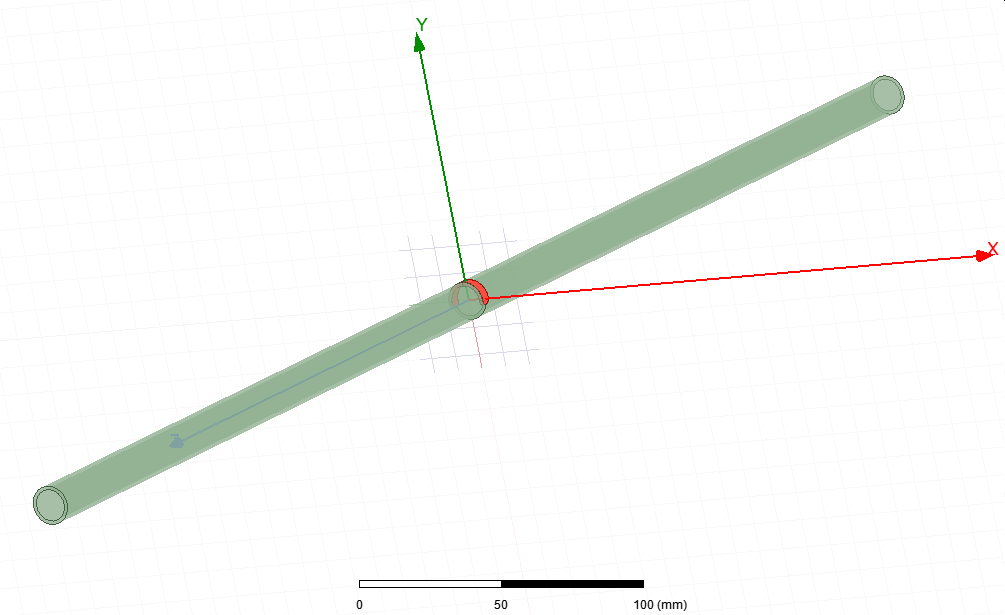
\includegraphics[width=0.9\linewidth]{img/waveguide.png}
    \caption{Entire waveguide geometry}
    \end{figure}
    
        \begin{figure}[H]
    \centering
    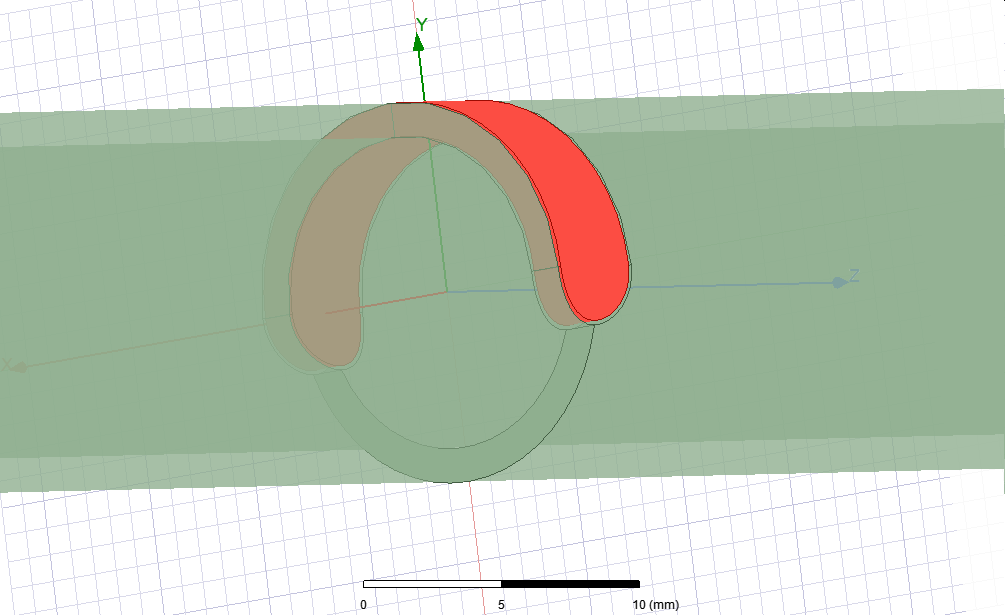
\includegraphics[width=0.9\linewidth]{img/cutout.png}
    \caption{5mm cutout with rounded boundary}
    \end{figure}
    
\subsection*{Background}
    
The purpose of this cutout is to give the operator of the experiment the ability to apply a voltage over the trap to clear the trap while also minimally disrupting the nominal operation of the experiment. This was chosen as the ideal design as the small cutout with the small gap and rounded edges prevent degenerate modes from being formed within it and this prevents power leaking from it. 

To validate this design we propagate waves from $18~$Ghz to $19~Ghz$ through the waveguide at both a vertical and a horizontal polarization and then measure the resulting S-parameters which indicate power transmission through the guide as a function of wavelength. These S-parameter plots are shown below

    \begin{figure}[H]
    \centering
    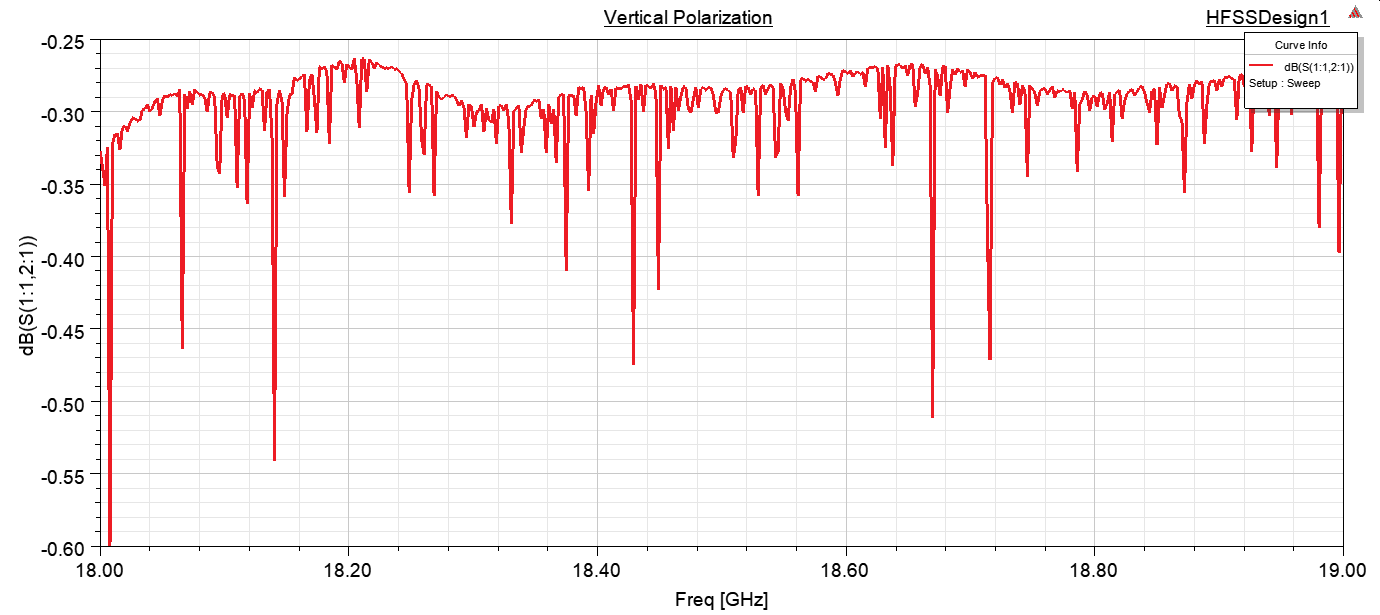
\includegraphics[width=\linewidth]{img/sparam_vert.png}
    \caption{S-Parameter for Vertically Polarized Wave Transmission}
    \end{figure}
    
    \begin{figure}[H]
    \centering
    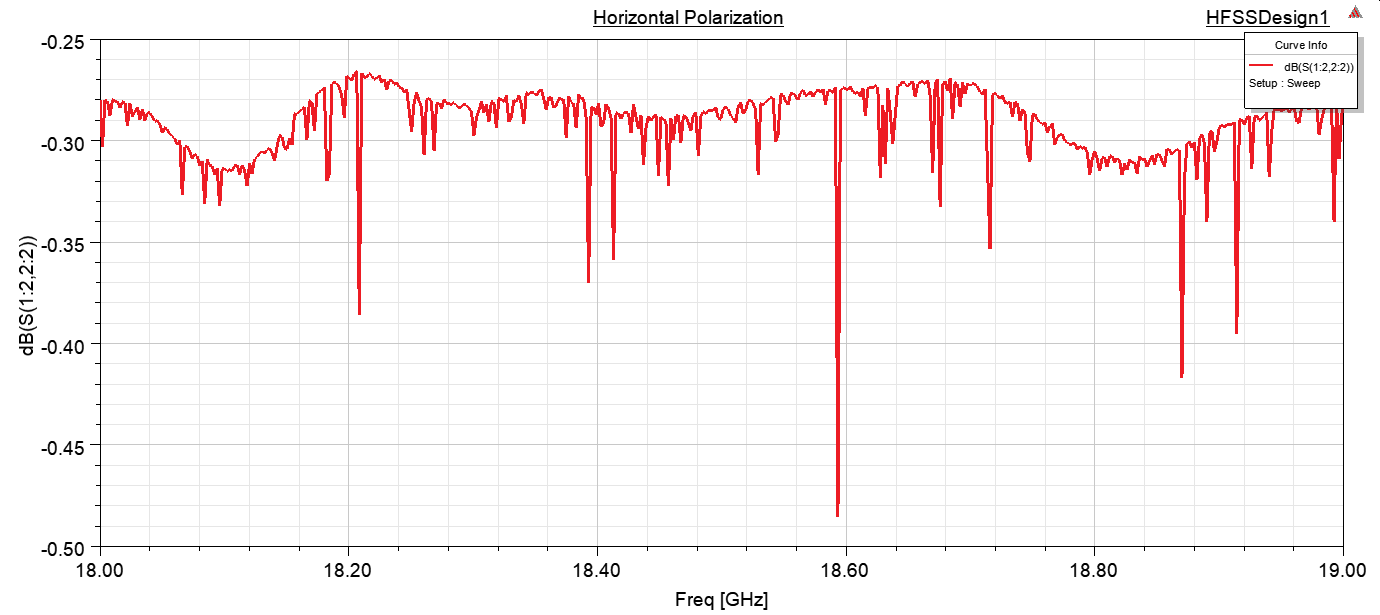
\includegraphics[width=\linewidth]{img/sparam_horiz.png}
    \caption{S-Parameter for Horizontally Polarized Wave Transmission }
    \end{figure}
    
    
We see on these plots that the attenuation never drops below $-0.6~$dB for either polarization which is acceptable and generally shows that no degenerate modes are being coupled to within the guide. 

We visualize the magnitude of the waves propagating through the waveguide during the simulation to identify any points of coupling or power leakage in the device. This visualization was generated using a wave with a driven frequency of $18.5~$Ghz 

    \begin{figure}[H]
    \centering
    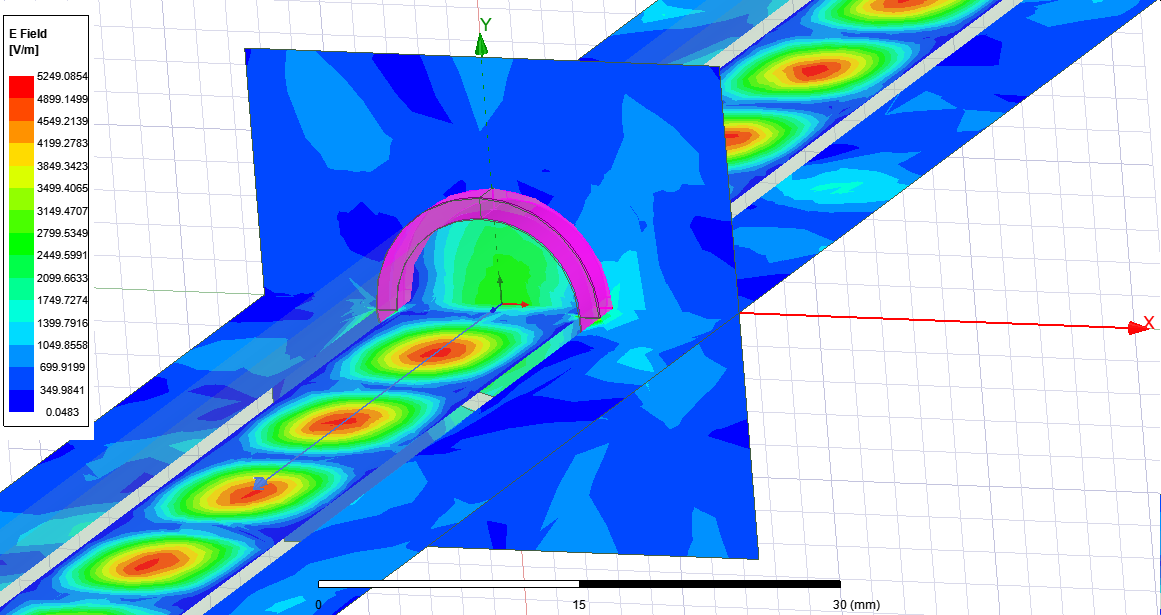
\includegraphics[width=\linewidth]{img/waves.png}
    \caption{Magnitude Plot of Propagating E-Field on Bisecting Planes through the Geometry}
    \end{figure}


We also visualize the static fields in the simulation to verify they are the magnitude and direction that we approximately expect them to be.

    \begin{figure}[H]
    \centering
    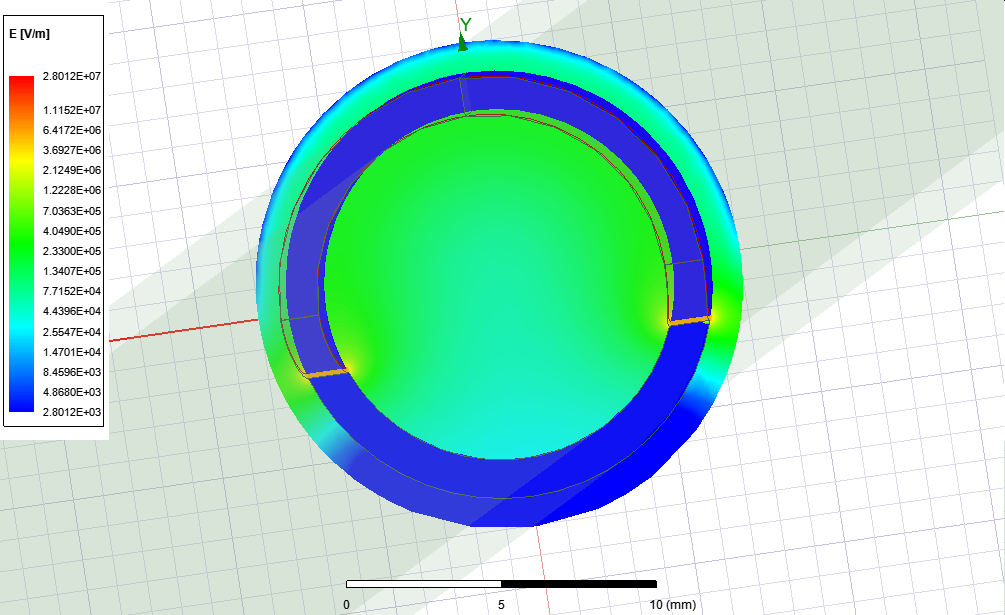
\includegraphics[width=0.9\linewidth]{img/emag_cutout.png}
    \caption{Magnitude Plot of E-Field on Cutout Cross-Section}
    \end{figure}
    
    \begin{figure}[H]
    \centering
    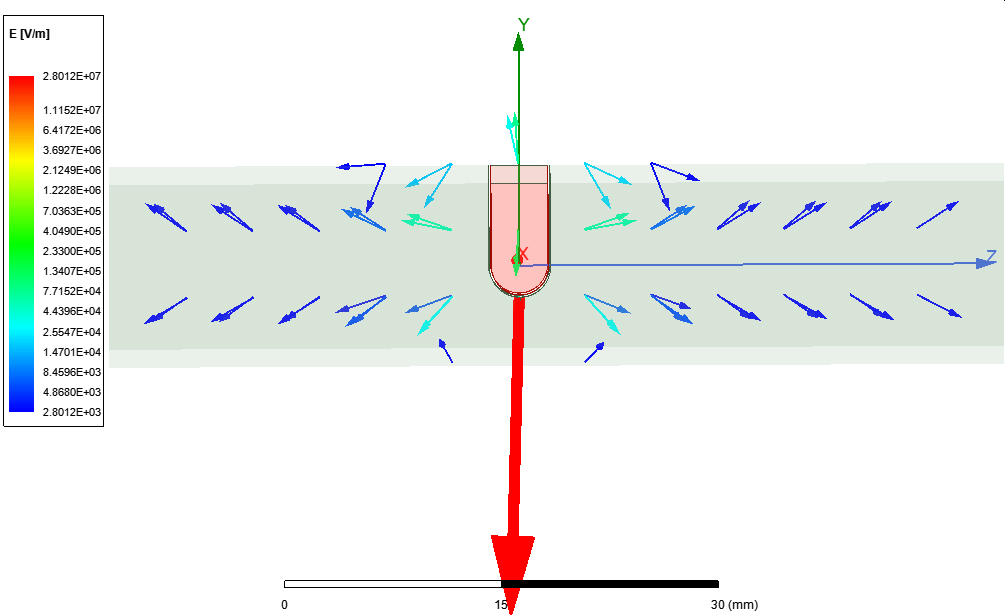
\includegraphics[width=0.9\linewidth]{img/evec_side.png}
    \caption{Vector Representation of E-Field from Side of Geometry}
    \end{figure}
    
These results support that the model will successfully propagate waves in the frequencies of interest without degenerate mode coupling and will also generate electric fields sufficient to clear the trap. 

\subsection*{Emptying Time Simulation}

We then export the generated E-field vectors from Ansys and import them into Kassiopeia replacing the global static electric field from the previous section. We then run the same emptying time simulation described above to achieve a realistic emptying time value. 

The emptying time histogram plot is shown below

    \begin{figure}[H]
    \centering
    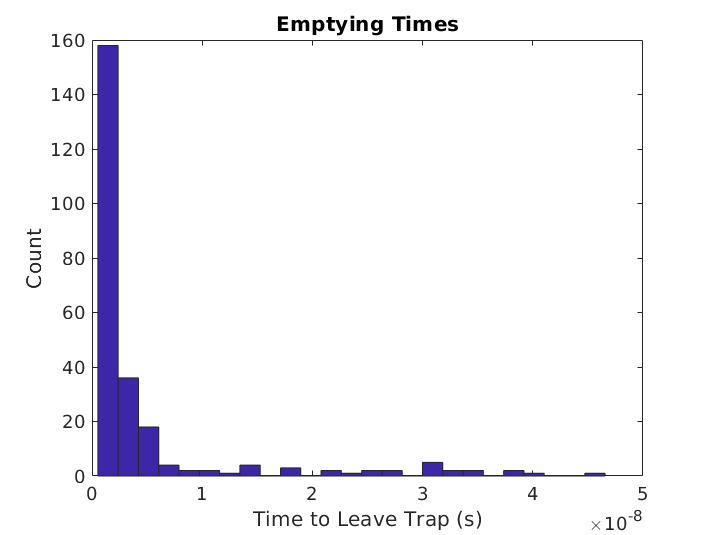
\includegraphics[width=0.7\linewidth]{img/emptying_mapped.png}
    \caption{Vector Representation of E-Field from Side of Geometry}
    \end{figure}
    
From this plot we observe that the bounds of the emptying times are similar to that of the static $2\times10^5~$V/m field with the exception that the vast majority of particles exit the trap within $10~$ns.

From this we conclude that the trap emptying geometry defined in this section is more than capable of emptying the circular waveguide of charged particles in a sufficiently short period of time while also causing little interference with the operation of the waveguide. 

\section{Appendix}

Code used to generate the figures in this document is accessible \href{https://github.com/robocoder99/CRES}{here}. The data used to generate these figures are available. Please contact the author, Alexander Allen (arallen4@ncsu.edu) for access. 


\end{document}

